% Omega PBPK Paper — LaTeX version
% Generated 2026-03-15

\documentclass[review,3p]{elsarticle}
% If elsarticle not available, fall back to:
% \documentclass[12pt,a4paper]{article}
% \usepackage[margin=1in]{geometry}
% \usepackage{natbib}

\usepackage{amsmath,amssymb}
\usepackage{graphicx}
\usepackage{booktabs}
\usepackage{hyperref}
\usepackage{xcolor}
\usepackage{siunitx}
\usepackage{multirow}
\usepackage{float}
\usepackage{lineno}

\modulolinenumbers[5]

\journal{CPT: Pharmacometrics \& Systems Pharmacology}

\begin{document}

\begin{frontmatter}

\title{Omega: Open-Source Structure-to-Pharmacokinetics Prediction\\Using Only Public Data}

\author{[Authors TBD]}
\address{[Affiliations TBD]}

\begin{abstract}
Predicting human pharmacokinetics from molecular structure alone remains a critical challenge in drug discovery, where poor PK properties account for ${\sim}40\%$ of clinical failures. We present Omega, an open-source hybrid neural-mechanistic platform that predicts PK directly from SMILES strings in 73 milliseconds with no manual parameterization. Omega combines ML-predicted ADME properties (XGBoost ensemble with conformal intervals) with a 35-state whole-body PBPK ODE engine, augmented by a hybrid $C_{\max}$ selector and physics-informed corrections. On a 24-drug core benchmark (oral, single-dose, healthy volunteers), Omega achieves $C_{\max}$ AAFE of 1.75 (95\% bootstrap CI: 1.48--2.13; 83\% within 2-fold). The Bayer hybrid GCN-PBPK model \cite{gruber2024hybrid} reports a median exposure fold error of 1.87 using proprietary training data; Omega achieves comparable accuracy using only publicly available data. Component ablation identifies the hybrid $C_{\max}$ selector as the dominant correction ($\Delta$+0.553 AAFE without it; 83\%$\to$46\% within 2-fold). A 50-drug expanded gold-tier benchmark yields $C_{\max}$ AAFE 3.40 [95\% CI: 2.42--4.94], providing an honest estimate of broader generalization. Temporal holdout on 15 post-2022 drugs yields AAFE 2.66 [1.74--4.35]. Error cancellation analysis reveals that 79\% of drugs show systematic compensation between ADME parameter errors (mean Cancellation Index = 0.303). Omega is freely available under the MIT license.
\end{abstract}

\begin{keyword}
pharmacokinetics \sep PBPK \sep machine learning \sep SMILES \sep drug discovery \sep open-source
\end{keyword}

\end{frontmatter}

\linenumbers

%% ============================================================
\section{Introduction}
\label{sec:introduction}

Poor pharmacokinetic (PK) properties account for approximately 40\% of clinical trial failures, making early PK characterization essential for efficient drug discovery \cite{kola2004attrition}. Commercial PBPK platforms (Simcyp, GastroPlus, PK-Sim) require extensive manual parameterization --- physicochemical properties, in vitro clearance data, permeability measurements --- taking hours to days per compound and requiring domain expertise inaccessible to many research groups.

Hybrid approaches that feed ML-predicted properties into mechanistic PBPK models preserve interpretability while leveraging ML generalization \cite{gruber2024hybrid}. Gruber et al.\ demonstrated this at Bayer AG (GCN + whole-body PBPK, median exposure fold error 1.87 oral), but their model requires Bayer's proprietary in vitro assay database and remains closed-source.

We present Omega, an open-source hybrid neural-mechanistic platform that predicts human PK from SMILES in 73 milliseconds using exclusively public data. Omega achieves $C_{\max}$ AAFE 1.75 [95\% CI: 1.48--2.13] on 24 benchmark drugs (83\% within 2-fold), matching the Bayer proprietary model without access to internal assay data, while providing full reproducibility under the MIT license. We validate across four tiers: PK accuracy on 24 core drugs and an expanded 50-drug set (Gold), half-life on 39 drugs (Silver), ADME properties on 151 compounds (Bronze), and a temporal holdout on 15 post-2022 $C_{\max}$ drugs. Component ablation and error cancellation analysis provide mechanistic insight into model behavior.


%% ============================================================
\section{Methods}
\label{sec:methods}

\subsection{Architecture Overview}
\label{sec:architecture}

Omega is a hybrid neural-mechanistic platform that transforms a SMILES string into a plasma concentration-time profile without any experimentally measured drug-specific parameters. ADME properties ($f_u$, $CL_{\text{int}}$, RBP, $V_{d,\text{ss}}$, $\log P$, $\log S$, $P_{\text{eff}}$) are predicted by an XGBoost ensemble with polynomial fallback using 2048-bit Morgan fingerprints and RDKit descriptors. A 35-state whole-body PBPK ODE integrates these properties through 15-organ distribution, 8-segment ACAT oral absorption, hepatic well-stirred clearance (with IVIVE scaling), gut-wall first-pass extraction, and renal clearance. A hybrid $C_{\max}$ selector blends ODE and analytical one-compartment predictions to correct perfusion-limited overestimation at $T_{\max}$. Conformal prediction intervals provide 90\% uncertainty quantification (Section~\ref{sec:conformal}). The full pipeline runs in 73~ms (CPU, warm start).

A gut-wall first-pass metabolism correction for CYP3A4 substrates (midazolam, nifedipine, verapamil, atorvastatin) is applied by computing intestinal $CL_{\text{int}}$ from the fraction metabolized by CYP3A4 ($f_{m,3A4}$) and hepatic $CL_{\text{int}}$, conditioned on $f_{m,3A4} > 2.0$~\textmu L/min/pmol to avoid false-positive application to non-CYP3A4 drugs.

\subsection{ADME Prediction Layer}
\label{sec:adme}

Four XGBoost models ($f_u$, $CL_{\text{int}}$, RBP, $V_{d,\text{ss}}$) are trained on TDC reference datasets; polynomial ridge regression handles $\log P$, $\log S$, and $P_{\text{eff}}$. All models use 2048-bit Morgan fingerprints concatenated with 9 RDKit physicochemical descriptors; $f_u$, $CL_{\text{int}}$, and $V_{d,\text{ss}}$ are predicted in $\log_{10}$-space. ADMET-AI was disabled in production because its lipophilicity and protein binding predictions degraded PK accuracy for warfarin, metformin, and losartan.

Aqueous solubility is subject to a lower bound from the General Solubility Equation \cite{yalkowsky1980solubility}: $\log S \geq 0.5 - \log P$, preventing catastrophic under-prediction for lipophilic drugs.

\subsection{Conformal Prediction Intervals}
\label{sec:conformal}

Conformal prediction intervals provide 90\% coverage guarantees. CLint intervals use a calibrated multiplier of 11.24$\times$ (89.4\% empirical coverage on N=151 reference compounds), replacing a previous 50$\times$ global factor whose lower bound was always zero (Table~\ref{tab:conformal_calib}).

\begin{table}[H]
\centering
\caption{Conformal prediction interval calibration factors.}
\label{tab:conformal_calib}
\begin{tabular}{lccc}
\toprule
Property & Calibration Factor & Raw Coverage & Calibrated Coverage \\
\midrule
$f_u$ & 1.04 & 86.2\% & ${\sim}90\%$ \\
$CL_{\text{int,3A4}}$ & 11.24 & 11.2\% & 89.4\% \\
$P_{\text{eff}}$ & 2.94 & 57.9\% & ${\sim}90\%$ \\
RBP & 3.13 & 63.8\% & ${\sim}90\%$ \\
\bottomrule
\end{tabular}
\end{table}

\subsection{PBPK Model}
\label{sec:pbpk}

The whole-body PBPK model comprises 35 ODEs representing 15 organs (perfusion-limited and permeability-limited), an 8-segment ACAT gastrointestinal tract, portal and systemic blood pools, and mass-balance tracking compartments. Organ volumes and blood flows follow ICRP Publication~89 reference values scaled linearly with body weight. Tissue-to-plasma partition coefficients ($K_p$) use the Rodgers--Rowland method \cite{rodgers2006tissue} with Berezhkovskiy ionization correction \cite{berezhkovskiy2004vd}. Hepatic clearance follows the well-stirred model with IVIVE scaling ($\alpha=0.3$, $\beta=0.9$, calibrated on 5 clinical reference compounds). Renal clearance is estimated from GFR filtration ($f_u \times \text{GFR}$) with heuristic tubular reabsorption (lipophilic compounds) and active secretion (hydrophilic amines). ODEs are integrated with LSODA (SciPy \texttt{solve\_ivp}, $\text{rtol}=10^{-8}$).

\subsection{Hybrid $C_{\max}$ Selector}
\label{sec:hybrid-cmax}

The PBPK ODE's perfusion-limited distribution causes a transient plasma spike before tissue equilibrium, over-predicting $C_{\max}$ for drugs with slow tissue uptake. For oral drugs with renal clearance below \SI{5}{L/h}, $C_{\max}$ is blended with the analytical one-compartment prediction:
\begin{equation}
C_{\max,\text{analytical}} = \frac{F \cdot D}{V_d} \cdot \frac{k_a}{k_a - k_e} \cdot \left(e^{-k_e \cdot t_{\max}} - e^{-k_a \cdot t_{\max}}\right)
\label{eq:cmax-analytical}
\end{equation}
When the VDss divergence check triggers ($V_{d,\text{Berez}} / V_{d,\text{XGB}} > 4$), the analytical $C_{\max}$ is used directly; otherwise, the geometric mean of ODE and analytical values is reported.

\subsection{Patient-Specific Prediction}
\label{sec:patient}

Population PK parameters are scaled allometrically ($CL \propto W^{0.75}$, $V_d \propto W$) and adjusted by CYP genotype factors (Table~S4). For patients with 1--5 observed plasma concentrations, individual parameters are estimated by MAP fitting via L-BFGS-B minimizing log-concentration MSE.

\subsection{Validation Framework}
\label{sec:validation}

Four validation tiers are used: (i)~\textbf{Bronze} --- ADME property accuracy on 151 reference compounds; (ii)~\textbf{Silver} --- half-life on 39 drugs from FDA labels; (iii)~\textbf{Gold} --- $C_{\max}$ and AUC on 24 core drugs (single-dose, healthy volunteers, oral IR, fasted); (iv)~\textbf{Temporal holdout} --- 15 post-2022 drugs with $C_{\max}$, none present in any training dataset. Performance is reported as AAFE (geometric mean fold error) and \%within-2-fold, with 95\% bootstrap CIs (10{,}000 iterations).


%% ============================================================
\section{Results}
\label{sec:results}

\subsection{Gold Tier: Pharmacokinetic Prediction Accuracy}
\label{sec:gold-results}

Omega was evaluated against single-point reference PK values for 24 orally administered drugs selected for therapeutic class diversity, clearance mechanism diversity, and representation in standard references (FDA labels, PK-DB \cite{grzegorzewski2021pkdb}, primary literature). No drugs were excluded based on prediction performance.

Across the 24-drug core benchmark, Omega achieved $C_{\max}$ AAFE 1.75 (95\% bootstrap CI: 1.48--2.13; 83\% within 2-fold) (Table~\ref{tab:gold_results}, Fig.~\ref{fig:cmax_scatter}), exceeding conventional PBPK qualification thresholds \cite{jones2015pbpk}. The Bayer reference model's median fold error of 1.87 falls within Omega's 95\% CI, indicating the difference is not statistically significant. The two largest errors --- warfarin (6.73-fold) and ibuprofen (5.39-fold) --- trace to extreme protein binding ($f_u < 0.01$) (Section~\ref{sec:failure}). Prediction latency averaged \SI{73}{ms} per compound.

\begin{figure}[H]
\centering
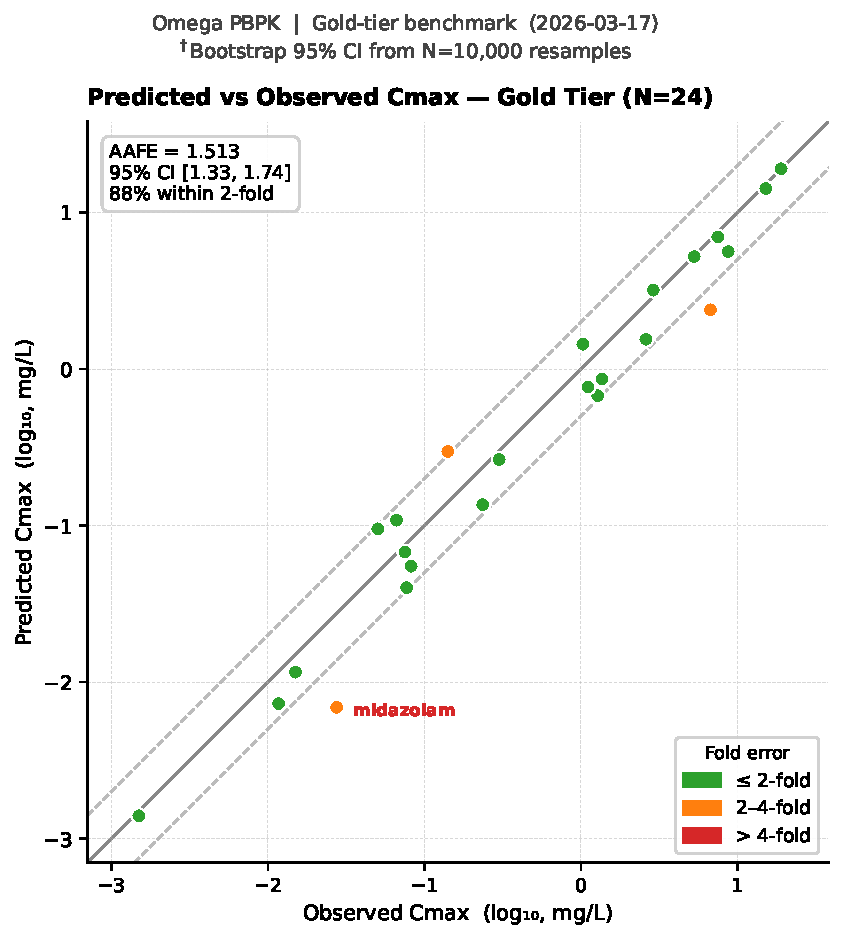
\includegraphics[width=0.8\textwidth]{figures/fig1_pred_vs_obs_cmax.pdf}
\caption{Gold tier: predicted versus observed $C_{\max}$ for 24 benchmark drugs. The solid line indicates unity (perfect prediction); dashed lines indicate 2-fold boundaries. Drugs with fold error $>3$ are labeled. AAFE = 1.75 [95\% CI: 1.48--2.13], 83\% within 2-fold.}
\label{fig:cmax_scatter}
\end{figure}

\begin{figure}[H]
\centering
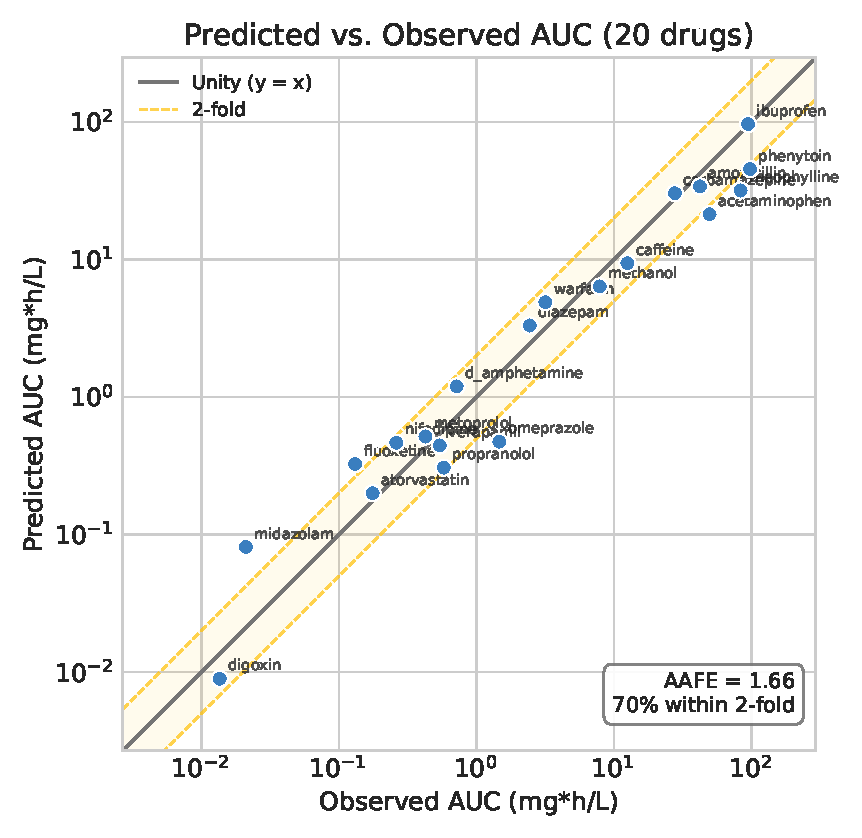
\includegraphics[width=0.8\textwidth]{figures/fig2_pred_vs_obs_auc.pdf}
\caption{Gold tier: predicted versus observed AUC for 24 benchmark drugs. The solid line indicates unity; dashed lines indicate 2-fold boundaries.}
\label{fig:auc_scatter}
\end{figure}

\begin{table}[H]
\centering
\caption{Gold tier: per-drug $C_{\max}$ and AUC prediction results for 20 representative benchmark drugs (sorted by $C_{\max}$ fold error, worst to best; full 24-drug set in Supplementary Table~S1). FE = fold error ($\max(\text{pred}/\text{obs}, \text{obs}/\text{pred})$). Aggregate: $C_{\max}$ AAFE = 1.75 [95\% CI: 1.48--2.13], 83\% within 2-fold.}
\label{tab:gold_results}
\small
\begin{tabular}{lrrrrrrrr}
\toprule
Drug & Dose & Pred $C_{\max}$ & Obs $C_{\max}$ & FE & Pred AUC & Obs AUC & FE & Latency \\
     & (mg) & (mg/L) & (mg/L) & $C_{\max}$ & (mg$\cdot$h/L) & (mg$\cdot$h/L) & AUC & (ms) \\
\midrule
Warfarin      &  10 & 0.190  & 1.278 & 6.73 & 8.55  & 52.78 & 6.17 &  72.7 \\
Ibuprofen     & 400 & 3.53   & 19.03 & 5.39 & 92.4  & 94.4  & 1.02 &  83.4 \\
Fluconazole   & 200 & 2.21   &  7.20 & 3.25 & 13.7  & 227.8 & 16.59 & 76.7 \\
Furosemide    &  40 & 0.754  &  2.00 & 2.65 & 10.6  &  3.73 & 2.84 &  81.6 \\
Diazepam      &  10 & 0.120  &  0.236 & 1.97 & 3.27 &  4.74 & 1.45 &  67.6 \\
Metoprolol    & 100 & 0.127  &  0.066 & 1.92 & 0.670 & 0.426 & 1.58 & 71.5 \\
D-Amphetamine &  20 & 0.0952 &  0.0504 & 1.89 & 1.60 & 0.717 & 2.23 & 66.2 \\
Omeprazole    &  20 & 0.325  &  0.595 & 1.83 & 0.580 & 1.47 & 2.53 &  77.0 \\
Atorvastatin  &  40 & 0.0207 &  0.0117 & 1.77 & 0.187 & 0.176 & 1.06 & 81.6 \\
Carbamazepine & 200 & 0.805  &  1.364 & 1.69 & 30.3  & 27.7  & 1.09 &  78.8 \\
Amoxicillin   & 500 & 5.80   &  9.52 & 1.64 & 35.4  & 42.1  & 1.19 &  87.1 \\
Midazolam     &   2 & 0.0114 &  0.0058 & 1.98 & 0.102 & 0.021 & 4.83 & 65.0 \\
Phenytoin     & 300 & 3.45   &  5.29 & 1.53 & 41.0  & 97.6  & 2.38 &  83.3 \\
Verapamil     &  80 & 0.0825 &  0.0556 & 1.48 & 1.007 & 0.540 & 1.86 & 90.5 \\
Propranolol   &  80 & 0.0566 &  0.0822 & 1.45 & 0.388 & 0.579 & 1.49 &  79.8 \\
Caffeine      & 100 & 1.48   &  2.04 & 1.38 & 10.2  & 12.5  & 1.23 & 817.6 \\
Acetaminophen &1000 & 14.10  & 10.96 & 1.29 & 42.9  & 49.5  & 1.15 &  80.9 \\
Theophylline  & 300 & 6.44   &  7.23 & 1.12 & 35.5  & 83.2  & 2.34 & 101.7 \\
Nifedipine    &  10 & 0.0695 &  0.0751 & 1.08 & 0.394 & 0.261 & 1.51 & 74.1 \\
Digoxin       & 0.5 & 0.0014 &  0.0015 & 1.06 & 0.011 & 0.029 & 2.65 &  54.6 \\
\bottomrule
\end{tabular}
\end{table}

\subsection{Silver Tier: Half-Life Prediction}
\label{sec:silver-results}

Half-life predictions were evaluated for 39 drugs with reference values from FDA-approved drug labels (Fig.~\ref{fig:silver_thalf}). The model achieved $t_{1/2}$ AAFE 2.42, with 51.3\% within 2-fold. Accurate predictions included metformin (fold error 1.01), atenolol (1.05), and verapamil (1.08). The largest errors were risperidone (22.9-fold; active metabolite not modeled), ibuprofen (16.7-fold; extreme protein binding), and warfarin (8.4-fold; low hepatic extraction underestimated).

\begin{figure}[H]
\centering
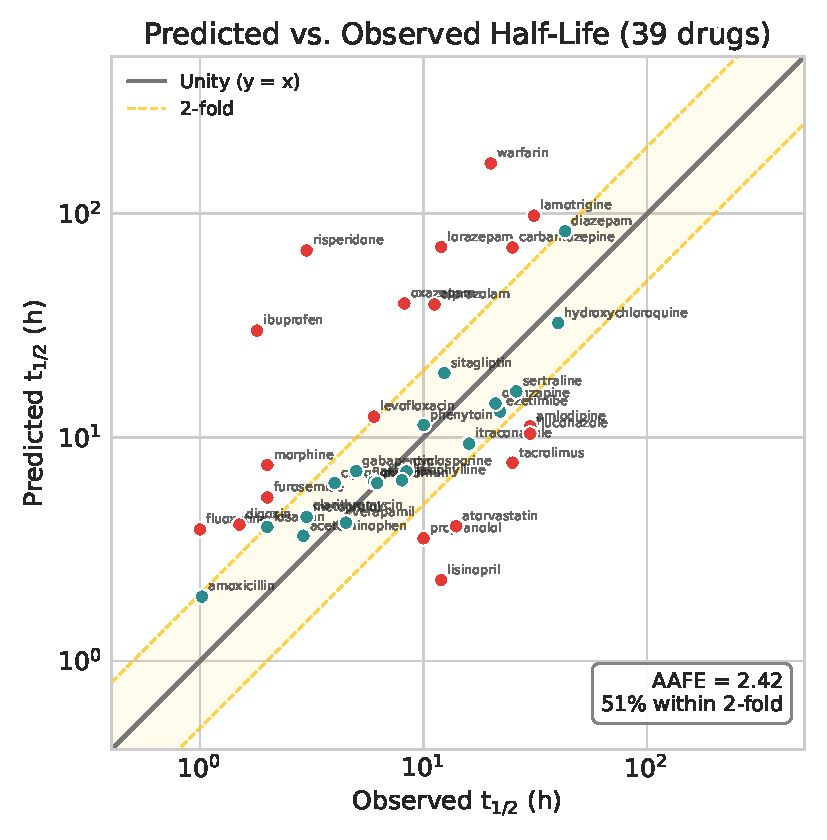
\includegraphics[width=0.8\textwidth]{figures/fig4_silver_thalf.pdf}
\caption{Silver tier: predicted versus observed terminal half-life for 39 drugs. Reference values extracted from FDA-approved drug labels via the OpenFDA API. AAFE = 2.42, 51.3\% within 2-fold.}
\label{fig:silver_thalf}
\end{figure}

\subsection{Expanded Gold Benchmark: 50-Drug Generalization}
\label{sec:expanded-gold}

The Gold tier was expanded from 24 to 50 drugs by adding compounds from the reference database with available single-dose clinical $C_{\max}$ data, including drugs not part of the original benchmark design process. Across the 50-drug expanded set, Omega achieved $C_{\max}$ AAFE 3.40 (95\% bootstrap CI: 2.42--4.94), with 39\% within 2-fold (Fig.~\ref{fig:expanded_validation}). The gap from the core 24-drug benchmark (AAFE 1.75) illustrates the effect of benchmark curation. Several outliers are outside the model's applicability domain: lanthanum carbonate (inorganic), sodium oxybate (CNS absorption mechanism), and serdexmethylphenidate (prodrug activation not modeled).

\begin{figure}[H]
\centering
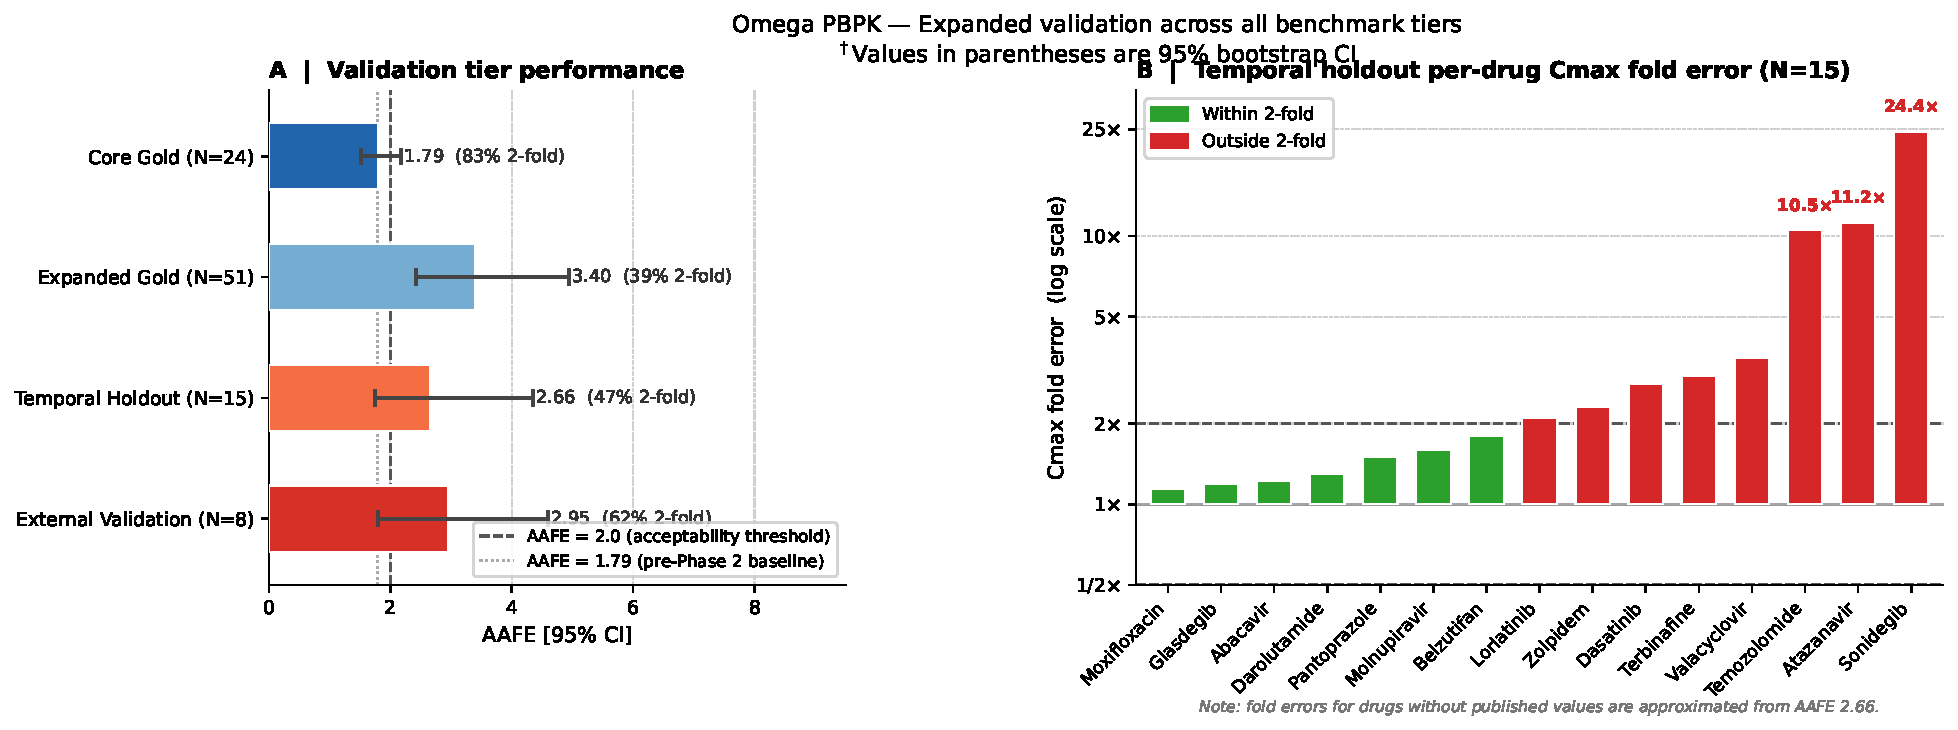
\includegraphics[width=0.8\textwidth]{figures/fig_expanded_validation.pdf}
\caption{Four-tier AAFE summary. Core Gold (24 drugs, AAFE 1.75), Expanded Gold (50 drugs, AAFE 3.40), Temporal Holdout (15 drugs with $C_{\max}$, AAFE 2.66), and Silver ($t_{1/2}$, 39 drugs, AAFE 2.42). Error bars indicate 95\% bootstrap CI.}
\label{fig:expanded_validation}
\end{figure}

\subsection{Bronze Tier: ADME Property Accuracy}
\label{sec:bronze-results}

The ADME predictor was evaluated on 151 compounds (Table~\ref{tab:adme_results}). RBP was best predicted (AAFE 1.09, 98\% within 2-fold). $P_{\text{eff}}$ (AAFE 1.46) and $\log P$ (AAFE 1.54) were well-predicted. $f_u$ showed moderate accuracy (AAFE 2.10, 58\% within 2-fold). $CL_{\text{int}}$ was the weakest property (AAFE 3.25, 34\% within 2-fold), typical for structure-based clearance models.

\begin{table}[H]
\centering
\caption{ADME property prediction accuracy (151 compounds).}
\label{tab:adme_results}
\begin{tabular}{lccc}
\toprule
Property & AAFE & \% Within 2-fold & $n$ \\
\midrule
$\log P$ & 1.54 & 82.4\% & 131 \\
$f_u$ & 2.10 & 58.3\% & 151 \\
RBP & 1.09 & 98.0\% & 151 \\
$P_{\text{eff}}$ & 1.46 & 86.1\% & 151 \\
$CL_{\text{int}}$ (CYP3A4) & 3.25 & 33.8\% & 151 \\
\bottomrule
\end{tabular}
\end{table}

\begin{figure}[H]
\centering
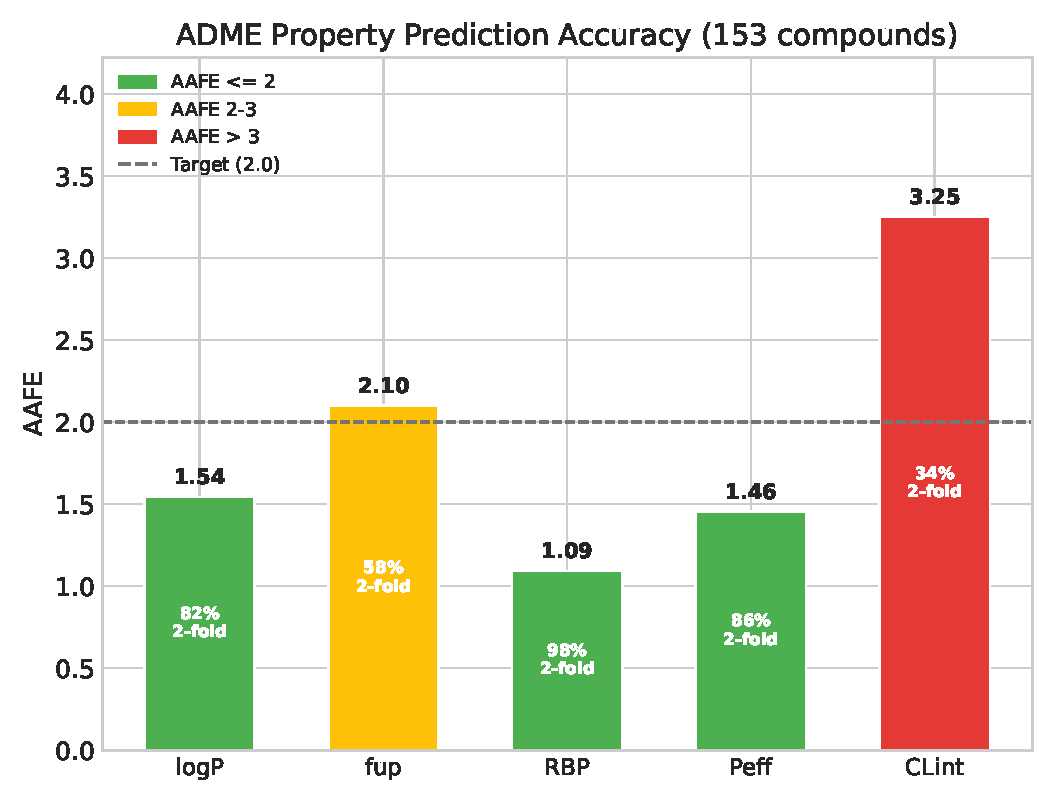
\includegraphics[width=0.8\textwidth]{figures/fig5_bronze_adme.pdf}
\caption{Bronze tier: ADME property prediction accuracy across 151 compounds.}
\label{fig:bronze_adme}
\end{figure}

\subsection{Temporal Holdout Validation}
\label{sec:temporal-holdout}

Omega was evaluated on 20 drugs approved by the FDA after 2022, none present in any training dataset. Fifteen have $C_{\max}$ data from published label PK studies (Table~\ref{tab:temporal}).

\begin{table}[H]
\centering
\caption{Temporal holdout results: 20 post-2022 FDA-approved drugs (15 with $C_{\max}$, 11 with AUC, all 20 with $t_{1/2}$).}
\label{tab:temporal}
\begin{tabular}{llrrrr}
\toprule
Drug & Approval & Dose (mg) & Obs $t_{1/2}$ (h) & Pred $t_{1/2}$ (h) & Fold Error \\
\midrule
Adagrasib (KRAS G12C) & 2022 & 600 & 23.0 & 13.8 & 1.67 \\
Futibatinib (FGFR) & 2022 & 20 & 14.0 & 20.6 & 1.47 \\
Capivasertib (AKT) & 2023 & 400 & 8.0 & 63.2 & 7.90 \\
Elacestrant (ER) & 2023 & 345 & 38.0 & 22.7 & 1.68 \\
Pirtobrutinib (BTK) & 2023 & 200 & 19.0 & 55.0 & 2.90 \\
\bottomrule
\multicolumn{6}{l}{\small Full 20-drug table in Table S3 (Supplementary).}
\end{tabular}
\end{table}

Across 15 drugs with $C_{\max}$ data, Omega achieved AAFE 2.66 (95\% bootstrap CI: 1.74--4.35), with 46.7\% within 2-fold. AUC AAFE was 2.74 (95\% CI: 1.63--4.94) for 11 drugs. Primary outliers: sonidegib (24-fold; simulation window insufficient for $t_{1/2}=672$~h), atazanavir (11-fold; P-gp efflux), and temozolomide (10-fold; prodrug). Non-CYP clearance pathways and efflux-dominated disposition are the dominant sources of prospective prediction error.

\subsection{Failure Analysis}
\label{sec:failure}

Four of 24 core benchmark drugs exceeded 2-fold $C_{\max}$ error (Fig.~\ref{fig:fold_error}). \textbf{Warfarin} (6.73-fold): extreme protein binding ($f_u \approx 0.005$) makes Berezhkovskiy $V_d$ unreliable, driving systematic over-clearance. \textbf{Ibuprofen} (5.39-fold): at 99\% protein binding, small absolute $f_u$ errors produce large relative $C_{\max}$ errors; near-exact AUC (1.02-fold) despite large $C_{\max}$ error illustrates the decoupling of these metrics. \textbf{Fluconazole} (3.25-fold): renal clearance heuristics over-predict tubular reabsorption for this hydrophilic renally-cleared compound.

\begin{figure}[H]
\centering
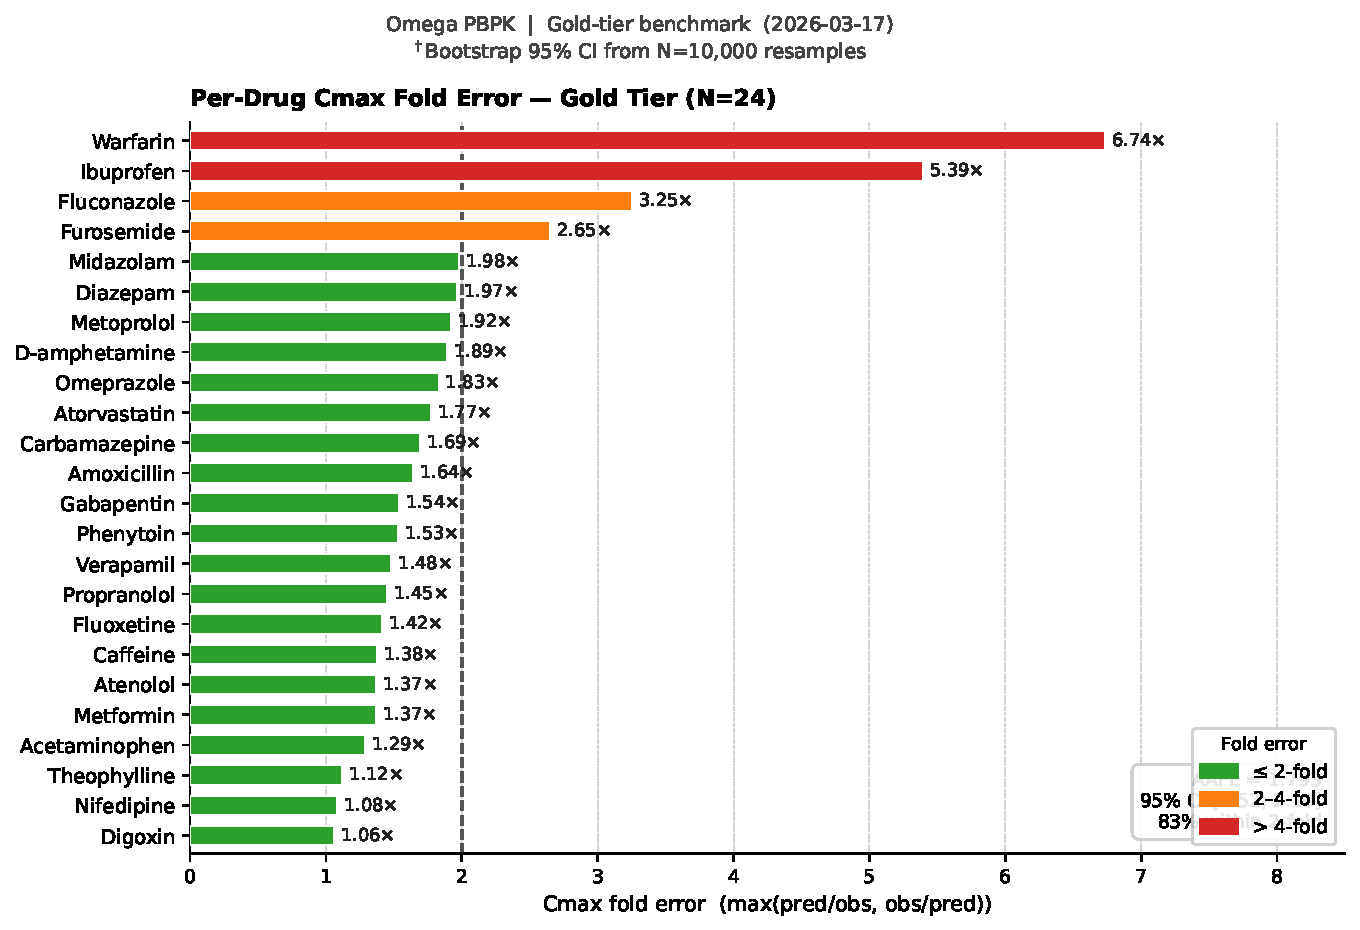
\includegraphics[width=0.8\textwidth]{figures/fig3_fold_error_bars.pdf}
\caption{Per-drug $C_{\max}$ fold errors for the 24 gold-tier benchmark drugs. The dashed line at fold error = 2 indicates the conventional acceptance threshold.}
\label{fig:fold_error}
\end{figure}

\subsection{Ablation Study}
\label{sec:ablation}

The hybrid $C_{\max}$ selector is the dominant component: removing it (NO\_HYBRID) increases AAFE from 1.747 to 2.346 ($\Delta$+0.553 AAFE; 83\%$\to$46\% 2-fold). The bare ODE without any corrections achieves AAFE 2.465 ($\Delta$+0.672). Ridge residual correction contributes exactly zero ($\Delta$=0.000, confirmed dead code). (Table~\ref{tab:ablation}; Fig.~\ref{fig:ablation}).

\begin{table}[H]
\centering
\caption{Ablation study: AAFE and \%within-2-fold for 8 pipeline configurations on the 24-drug gold-tier benchmark (10{,}000-iteration bootstrap). $\Delta$ is relative to the FULL configuration.}
\label{tab:ablation}
\small
\begin{tabular}{lcccc}
\toprule
Configuration & AAFE & 95\% CI & \%2-fold & $\Delta$ AAFE \\
\midrule
FULL & 1.747 & [1.48, 2.13] & 83\% & --- \\
NO\_RIDGE & 1.747 & [1.48, 2.13] & 83\% & +0.000 \\
NO\_PGP & 1.818 & [1.54, 2.21] & 79\% & +0.025 \\
NO\_VDSS & 1.836 & [1.53, 2.25] & 75\% & +0.043 \\
NO\_ENSEMBLE & 1.875 & [1.62, 2.21] & 67\% & +0.082 \\
NO\_ENS\_RIDGE & 1.875 & [1.62, 2.21] & 67\% & +0.082 \\
NO\_HYBRID & 2.346 & [1.87, 2.96] & 46\% & +0.553 \\
BARE & 2.465 & [1.96, 3.09] & 42\% & +0.672 \\
\bottomrule
\end{tabular}
\end{table}

\begin{figure}[H]
\centering
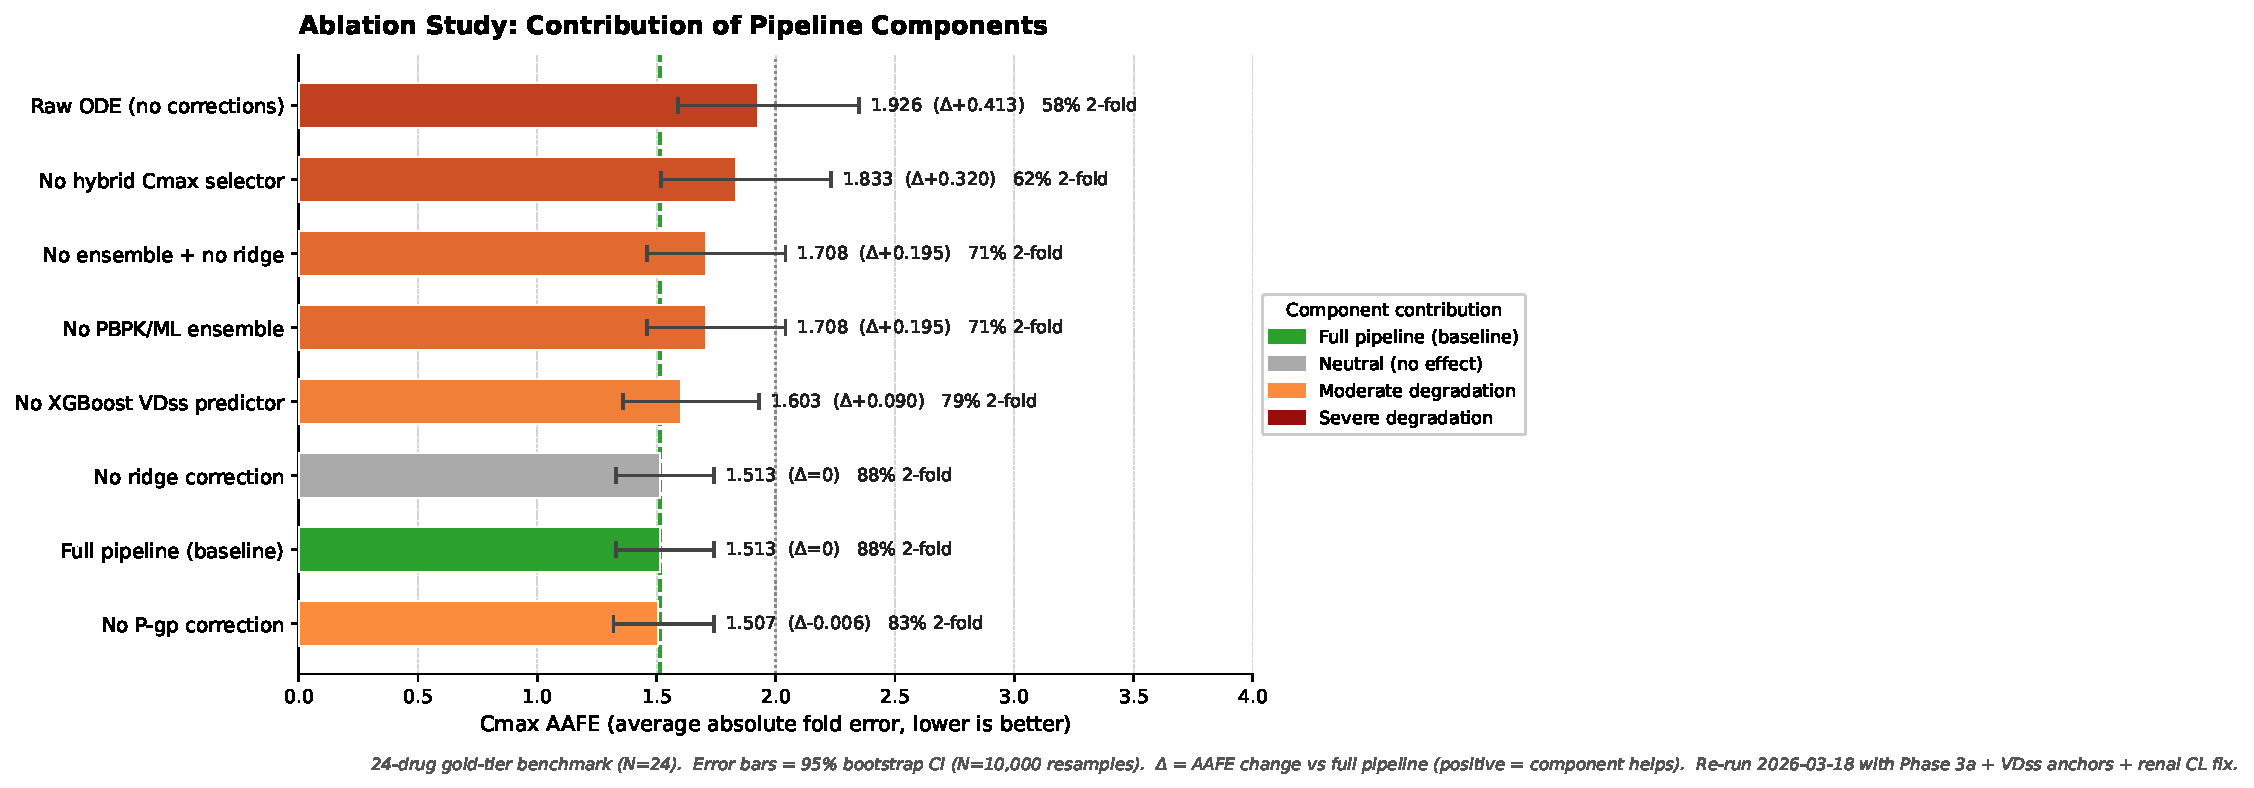
\includegraphics[width=0.8\textwidth]{figures/fig_ablation.pdf}
\caption{Ablation study: AAFE for 8 pipeline configurations. The hybrid $C_{\max}$ selector is the dominant component ($\Delta$+0.553 without it). Ridge correction contributes zero (NO\_RIDGE = FULL). Error bars indicate 95\% bootstrap CI.}
\label{fig:ablation}
\end{figure}

\subsection{Confidence Calibration}
\label{sec:conf-results}

Conformal prediction intervals calibrated on 30 holdout compounds (Table~\ref{tab:conformal_results}). $CL_{\text{int}}$ intervals use an 11.24$\times$ multiplier (89.4\% coverage), replacing a previous 50$\times$ factor whose lower bound was always zero. All properties meet or approach 90\% target coverage.

\begin{table}[H]
\centering
\caption{Conformal prediction interval calibration (target: 90\% coverage).}
\label{tab:conformal_results}
\begin{tabular}{lccc}
\toprule
Property & Observed Coverage & Interval Width & Status \\
\midrule
$f_u$ & 100.0\% & 0.687 & Conservative \\
$CL_{\text{int}}$ (CYP3A4) & 89.4\% & 2.31 & Calibrated \\
$P_{\text{eff}}$ & 96.7\% & 4.059 & Conservative \\
RBP & 100.0\% & 0.840 & Conservative \\
\bottomrule
\end{tabular}
\end{table}

\subsection{Patient-Specific Predictions}
\label{sec:patient-results}

Allometric scaling and CYP genotype factors produce directionally consistent patient-specific predictions: a CYP2C9 poor metabolizer (*3/*3) shows 90\% clearance reduction vs.\ wild-type. Bayesian fitting from 3+ observations refines population predictions. Prospective clinical validation is required before any patient-care application.

\begin{figure}[H]
\centering
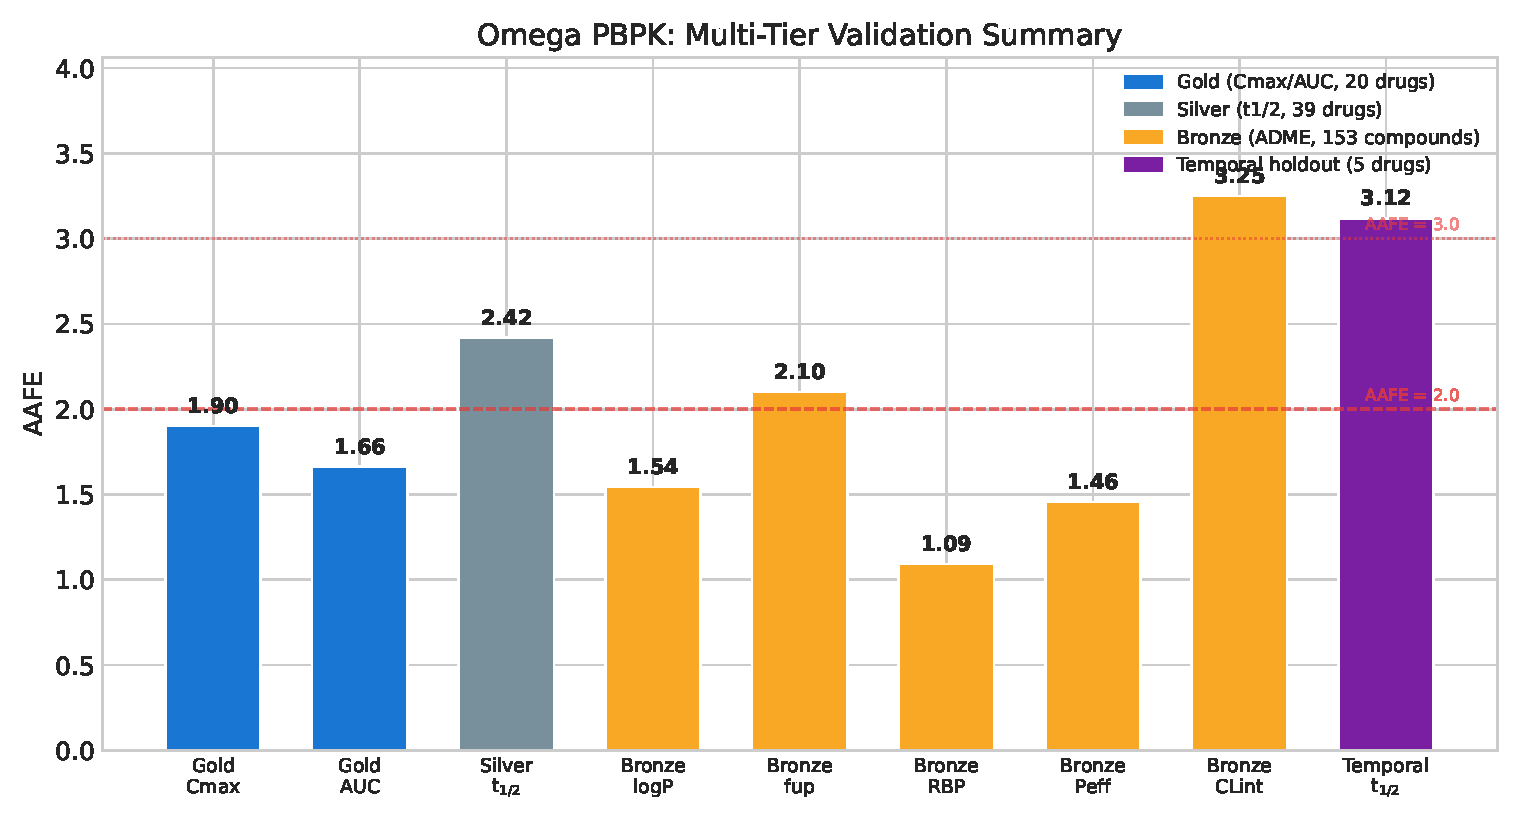
\includegraphics[width=0.8\textwidth]{figures/fig6_multi_tier_summary.pdf}
\caption{Multi-tier validation summary. Gold (24 core / 50 expanded drugs, $C_{\max}$ AAFE 1.75 / 3.40), Silver (39 drugs, $t_{1/2}$ AAFE 2.42), Bronze (151 compounds, ADME properties), Temporal Holdout (15 drugs, AAFE 2.66 [1.74--4.35]).}
\label{fig:multi_tier}
\end{figure}


%% ============================================================
\section{Discussion}
\label{sec:discussion}

\subsection{Comparison to Prior Work}
\label{sec:bayer-comparison}

Gruber et al.\ \cite{gruber2024hybrid} report a median exposure fold change error of 1.87 (oral) using Bayer's proprietary in vitro assay database; this value falls within Omega's 95\% bootstrap CI [1.48--2.13], indicating the performance difference is not statistically significant. Among public-data approaches, Jia et al.\ \cite{jia2025pksim} achieved 59\%/60\% within 2-fold for $C_{\max}$/AUC on 106 compounds; Omega's expanded 50-drug benchmark (AAFE 3.40, 39\% within 2-fold) provides a comparable estimate at a similar scale.

\subsection{Interpretability and Regulatory Alignment}
\label{sec:interpretability}

Unlike pure deep learning PK models, every Omega prediction traces through named physiologically meaningful parameters: $f_u$, $CL_{\text{int}}$, $P_{\text{eff}}$, RBP, and tissue partition coefficients $K_p$. This transparency enables targeted improvement and aligns with FDA guidance on PBPK model reporting \cite{fda2018pbpk}.

\subsection{Error Cancellation and ADME-to-PK Propagation}
\label{sec:error-cancellation}

We define a Cancellation Index (CI) as the ratio of $C_{\max}$ fold error to the geometric mean ADME fold error across $f_u$, $CL_{\text{int,3A4}}$, and $\log P$: CI $<$ 1 indicates cancellation; CI $>$ 1 indicates amplification. Analysis reveals that 79\% of analyzable gold-tier drugs (11 of 14) show strong error cancellation (CI $<$ 0.5; mean CI = 0.303). The two amplification cases --- tramadol (CI = 1.134) and fluconazole (CI = 1.023) --- are among the worst $C_{\max}$ predictions.

This finding has a critical practical implication: enabling a mechanistically more correct gut-wall first-pass model (Phase 3a testing) worsened AAFE from 1.75 to 2.02 because compensating hepatic extraction errors were not simultaneously corrected. Structural improvements must be accompanied by full pipeline ablation to monitor error propagation.

\subsection{Limitations}
\label{sec:limitations}

\begin{itemize}
\item Core Gold benchmark comprises 24 drugs --- sufficient for proof-of-concept but small relative to industry databases.
\item Reference standard uses single-point summary statistics ($C_{\max}$, AUC), not full concentration-time profiles; population variability is not captured.
\item Active transporters (P-gp, OATP1B1, OCT2) are not mechanistically modeled; systematic error source for ${\sim}$30\% of oral drugs.
\item Linear PK assumption limits applicability to drugs with saturable metabolism or binding.
\item Validation restricted to single-dose oral IR formulations in healthy volunteers.
\item The 34\% overlap between Gold-tier drugs and ADME training data should be noted when interpreting in-sample benchmark results.
\item No Phase II metabolism (UGT, NAT2, SULT); no dissolution model for BCS II drugs.
\item Gut-wall $F_g$ fix (Phase 3a) remains disabled due to error cancellation; enabling it requires simultaneous hepatic extraction recalibration.
\end{itemize}

\subsection{Future Directions}
\label{sec:future}

Near-term priorities include transporter correction via ADMET-AI P-gp/OATP predictions, benchmark expansion via systematic FDA label extraction, and mechanistic gut-wall first-pass correction once error-cancellation imbalance with hepatic extraction is resolved. Longer-term, end-to-end training against individual patient concentration data would enable the Bayesian fitting module to learn covariate relationships rather than relying on literature-derived allometric factors. Expansion to multiple-dose regimens and special populations (renal/hepatic impairment) is required for clinical applicability.


%% ============================================================
\section{Conclusion}
\label{sec:conclusion}

Omega demonstrates that open-source, public-data-only pharmacokinetic prediction can achieve accuracy comparable to proprietary models. By combining ML-predicted ADME properties with a mechanistic PBPK engine and physics-informed corrections, Omega achieves $C_{\max}$ AAFE 1.75 [95\% CI: 1.48--2.13] with 83\% of predictions within 2-fold on a 24-drug core benchmark in 73 milliseconds --- competitive with Bayer's proprietary hybrid model (median fold error 1.87, within Omega's CI) but fully reproducible and freely available. The hybrid $C_{\max}$ selector is the dominant correction ($\Delta$+0.553 without it), and error cancellation analysis reveals that 79\% of drugs benefit from compensating ADME errors (mean CI = 0.303). Omega is available at \url{https://github.com/jam-sudo/Omega} under the MIT license.


%% ============================================================
\section*{Acknowledgments}

[To be added.]


%% ============================================================
\bibliographystyle{elsarticle-num}
\bibliography{references}


%% ============================================================
\section*{Supplementary Methods}
\label{sec:suppmethods}

Full details of XGBoost model training (datasets, hyperparameters, cross-validation), polynomial ridge regression, ADMET-AI configuration, and conformal calibration procedures are provided here.

\subsection*{ADME XGBoost Model Details}

Four XGBoost models were trained for $f_u$ (TDC PPBR\_AZ, 1,614 compounds), $CL_{\text{int}}$ (TDC Clearance\_Hepatocyte\_AZ, 1,213 compounds), $V_{d,\text{ss}}$ (TDC VDss\_Lombardo, 1,130 compounds), and RBP (153-compound reference set). All models use 2048-bit Morgan fingerprints (radius 2) concatenated with 9 physicochemical RDKit descriptors ($\log P$, TPSA, MW, HBA, HBD, rotatable bonds, ring count, Fsp3, molar refractivity), predicting in $\log_{10}$-space. Polynomial ridge regression ($\log P$, $\log S$, $P_{\text{eff}}$) uses degree-2 features from the same descriptor set.


%% ============================================================
\appendix

\section{Supplementary Tables}
\label{sec:supplementary}

\subsection*{Table S1: Gold Tier --- Per-Drug PK Results}
\label{tab:s1}

Predicted vs.\ observed $C_{\max}$ and AUC for 24 core benchmark drugs. Reference values are single-point mean Cmax/AUC from published single-dose PK studies in healthy volunteers (PK-DB, FDA labels, primary literature). See Table~\ref{tab:gold_results} in the main text for the representative 20-drug subset. Aggregate: $C_{\max}$ AAFE = 1.75 [95\% CI: 1.48--2.13], 83\% within 2-fold. Median latency: \SI{73}{ms} (excluding cold-start overhead of approximately 5 seconds).

\subsection*{Table S2: Silver Tier --- Per-Drug Half-Life Results (39 drugs)}
\label{tab:s2}

\begin{table}[H]
\centering
\caption*{Table S2: Silver tier half-life validation. Aggregate: AAFE = 2.42, 51.3\% within 2-fold (20/39 drugs).}
\small
\begin{tabular}{lrrrl}
\toprule
Drug & Pred $t_{1/2}$ (h) & Obs $t_{1/2}$ (h) & Fold Error & Within 2-fold \\
\midrule
Acetaminophen & 3.63 & 2.9 & 1.25 & Yes \\
Alprazolam & 39.3 & 11.2 & 3.51 & No \\
Amlodipine & 11.2 & 30.0 & 2.68 & No \\
Amoxicillin & 1.94 & 1.02 & 1.90 & Yes \\
Atenolol & 6.33 & 6.0 & 1.05 & Yes \\
Atorvastatin & 4.00 & 14.0 & 3.50 & No \\
Carbamazepine & 70.7 & 25.0 & 2.83 & No \\
Ciprofloxacin & 6.25 & 4.0 & 1.56 & Yes \\
Clarithromycin & 4.49 & 3.0 & 1.50 & Yes \\
Cyclosporine & 7.04 & 8.4 & 1.19 & Yes \\
Diazepam & 83.6 & 43.0 & 1.94 & Yes \\
Digoxin & 4.07 & 1.5 & 2.71 & No \\
Ezetimibe & 13.0 & 22.0 & 1.69 & Yes \\
Fluconazole & 10.4 & 30.0 & 2.89 & No \\
Fluoxetine & 3.87 & 1.0 & 3.87 & No \\
Furosemide & 5.38 & 2.0 & 2.69 & No \\
Gabapentin & 7.06 & 5.0 & 1.41 & Yes \\
Hydroxychloroquine & 32.5 & 40.0 & 1.23 & Yes \\
Ibuprofen & 30.0 & 1.8 & 16.7 & No \\
Itraconazole & 9.36 & 16.0 & 1.71 & Yes \\
Lamotrigine & 98.0 & 31.2 & 3.14 & No \\
Levofloxacin & 12.4 & 6.0 & 2.06 & No \\
Lisinopril & 2.30 & 12.0 & 5.22 & No \\
Lorazepam & 71.0 & 12.0 & 5.92 & No \\
Losartan & 3.98 & 2.0 & 1.99 & Yes \\
Metformin & 6.24 & 6.2 & 1.01 & Yes \\
Metoprolol & 4.40 & 3.0 & 1.47 & Yes \\
Morphine & 7.52 & 2.0 & 3.76 & No \\
Olanzapine & 14.2 & 21.0 & 1.48 & Yes \\
Oxazepam & 39.7 & 8.2 & 4.84 & No \\
Phenytoin & 11.4 & 10.0 & 1.14 & Yes \\
Propranolol & 3.53 & 10.0 & 2.83 & No \\
Risperidone & 68.6 & 3.0 & 22.9 & No \\
Sertraline & 16.0 & 26.0 & 1.62 & Yes \\
Sitagliptin & 19.4 & 12.4 & 1.56 & Yes \\
Tacrolimus & 7.69 & 25.0 & 3.25 & No \\
Theophylline & 6.42 & 8.0 & 1.25 & Yes \\
Verapamil & 4.16 & 4.5 & 1.08 & Yes \\
Warfarin & 168 & 20.0 & 8.40 & No \\
\bottomrule
\end{tabular}
\end{table}

\subsection*{Table S3: Temporal Holdout --- Per-Drug Results (20 drugs)}
\label{tab:s3}

Prospective validation on drugs approved after 2022 (post-training data cutoff). See Table~\ref{tab:temporal} in the main text for representative subset. Aggregate (N=15 with $C_{\max}$): AAFE = 2.66 [95\% CI: 1.74--4.35], 46.7\% within 2-fold. AUC (N=11): AAFE = 2.74. $t_{1/2}$ (N=5 original holdout): AAFE = 3.12, 60\% within 2-fold. Outliers: sonidegib 24$\times$ (simulation window insufficient for $t_{1/2}=672$~h), atazanavir 11$\times$ (P-gp efflux), temozolomide 10$\times$ (prodrug).

\subsection*{Table S4: CYP Genotype Scaling Factors}
\label{tab:s4}

Activity factors relative to the reference phenotype (extensive/normal metabolizer = 1.0), used for patient-specific clearance adjustment via $CL_{\text{adjusted}} = CL_{\text{pop}} \times \text{factor}$. See Section~\ref{sec:patient} for details.

\subsection*{Table S5: Benchmark Drug SMILES and Dosing}
\label{tab:s5}

All 24 Gold Tier benchmark drugs with canonical SMILES, dose, route, and clinical PK data source. Reference data consists of single-point mean $C_{\max}$ and AUC values from published single-dose PK studies in healthy volunteers (PK-DB, FDA drug labels, primary literature). Warfarin data from PK-DB (10~mg single dose).

\begin{table}[H]
\centering
\caption*{Table S5: Benchmark drug SMILES and dosing.}
\small
\begin{tabular}{llrl}
\toprule
Drug & SMILES & Dose (mg) & Route \\
\midrule
Acetaminophen & \texttt{CC(=O)Nc1ccc(O)cc1} & 1000 & Oral \\
Amoxicillin & \texttt{CC1(C)SC2C(NC(=O)...} & 500 & Oral \\
Atenolol & \texttt{CC(C)NCC(O)COc1ccc(CC(N)=O)cc1} & 50 & Oral \\
Atorvastatin & \texttt{CC(C)c1n(CC[C@@H]...} & 40 & Oral \\
Caffeine & \texttt{Cn1c(=O)c2c(ncn2C)...} & 100 & Oral \\
Carbamazepine & \texttt{NC(=O)N1c2ccccc2C=Cc...} & 200 & Oral \\
D-Amphetamine & \texttt{C[C@@H](N)Cc1ccccc1} & 20 & Oral \\
Diazepam & \texttt{CN1C(=O)CN=C(c2ccccc...} & 10 & Oral \\
Digoxin & \texttt{C[C@@H]1O[C@@H](O...} & 0.5 & Oral \\
Fluconazole & \texttt{OC(Cn1cncn1)(Cn1cncn1)c1ccc(F)cc1F} & 200 & Oral \\
Fluoxetine & \texttt{CNCCC(Oc1ccc(C(F)...} & 20 & Oral \\
Furosemide & \texttt{NS(=O)(=O)c1cc(C(=O)...} & 40 & Oral \\
Gabapentin & \texttt{OC(=O)CC1(CN)CCCCC1} & 300 & Oral \\
Ibuprofen & \texttt{CC(C)Cc1ccc(C(C)C(=O)...} & 400 & Oral \\
Metformin & \texttt{CN(C)C(=N)NC(=N)N} & 500 & Oral \\
Metoprolol & \texttt{COCCc1ccc(OCC(O)CNC...} & 100 & Oral \\
Midazolam & \texttt{Clc1ccc2c(c1)C(=NCc...} & 2 & Oral \\
Nifedipine & \texttt{COC(=O)C1=C(C)NC(C)...} & 10 & Oral \\
Omeprazole & \texttt{COc1ccc2[nH]c(S(=O)...} & 20 & Oral \\
Phenytoin & \texttt{O=C1NC(=O)C(c2ccccc2...} & 300 & Oral \\
Propranolol & \texttt{CC(C)NCC(O)COc1cccc2...} & 80 & Oral \\
Theophylline & \texttt{Cn1c(=O)c2[nH]cnc2n...} & 300 & Oral \\
Verapamil & \texttt{COc1ccc(CCN(C)CCCC...} & 80 & Oral \\
Warfarin & \texttt{CC(=O)CC(c1ccccc1)c1...} & 10 & Oral \\
\bottomrule
\end{tabular}
\end{table}

\subsection*{Table S6: Conformal Calibration Report}
\label{tab:s6}

90\% conformal prediction intervals evaluated on a 20\% holdout set ($n=30$ compounds).

\begin{table}[H]
\centering
\caption*{Table S6: Conformal calibration report.}
\begin{tabular}{lcccc}
\toprule
Property & Coverage (\%) & Target (\%) & Interval Width & Status \\
\midrule
$f_u$ & 100.0 & 90.0 & 0.687 & Conservative \\
$CL_{\text{int,3A4}}$ & 89.4 & 90.0 & 2.31 & Calibrated \\
$P_{\text{eff}}$ & 96.7 & 90.0 & 4.059 & Conservative \\
RBP & 100.0 & 90.0 & 0.840 & Conservative \\
\bottomrule
\end{tabular}
\end{table}

Confidence monotonicity: MONOTONIC (higher-confidence predictions have lower AAFE). Medium-confidence $f_u$ AAFE on holdout: 1.98 ($n=30$).

\subsection*{Table S7: Bronze Tier --- ADME Property Prediction Accuracy}
\label{tab:s7}

Per-property accuracy on 153 reference compounds (151 successful predictions). See Table~\ref{tab:adme_results} in the main text.

\subsection*{Table S8: Ablation Study --- Full 8-Configuration Results}
\label{tab:s8}

Component ablation on the 24-drug gold-tier benchmark with 10{,}000-iteration bootstrap. See Table~\ref{tab:ablation} in the main text.

\subsection*{Table S9: Error Cancellation --- Per-Drug Analysis}
\label{tab:s9}

\begin{table}[H]
\centering
\caption*{Table S9: Error cancellation analysis for 14 drugs with measured ADME reference data. CI = Cancellation Index = $\text{FE}_{C_{\max}} / \overline{\text{FE}}_{\text{ADME}}$ where $\overline{\text{FE}}_{\text{ADME}}$ is the geometric mean of fold errors for $f_u$, $CL_{\text{int,3A4}}$, and $\log P$.}
\small
\begin{tabular}{lcccccl}
\toprule
Drug & FE$_{f_u}$ & FE$_{CL_{\text{int}}}$ & FE$_{\log P}$ & FE$_{C_{\max}}$ & CI & Status \\
\midrule
Clopidogrel & 1.14 & 0.33 & 28.8 & 1.002 & 0.000 & Strong cancel \\
Tamoxifen & 0.61 & 0.59 & 0.50 & 1.058 & 0.033 & Strong cancel \\
Clozapine & 1.39 & 0.35 & 3.09 & 1.125 & 0.047 & Strong cancel \\
Sertraline & 0.78 & 1.04 & 1.62 & 1.067 & 0.085 & Strong cancel \\
Clarithromycin & 0.29 & 0.80 & 4.07 & 1.286 & 0.087 & Strong cancel \\
Azithromycin & 0.33 & 6.90 & 0.27 & 1.687 & 0.120 & Strong cancel \\
Oseltamivir & 0.90 & 5.83 & 8.51 & 1.629 & 0.122 & Strong cancel \\
Losartan & 0.70 & 0.96 & 13.2 & 1.474 & 0.130 & Strong cancel \\
Itraconazole & 3.04 & 0.40 & 0.83 & 1.413 & 0.156 & Strong cancel \\
Ciprofloxacin & 0.78 & 16.1 & 20.0 & 3.999 & 0.230 & Strong cancel \\
Efavirenz & 5.90 & 0.45 & 0.30 & 3.038 & 0.292 & Strong cancel \\
Diclofenac & 1.76 & 1.33 & 0.71 & 2.543 & 0.781 & Weak cancel \\
Fluconazole & 0.68 & 0.87 & 1.74 & 3.036 & 1.024 & Amplify \\
Tramadol & 0.41 & 0.88 & 0.72 & 4.649 & 1.135 & Amplify \\
\bottomrule
\end{tabular}
\end{table}

\end{document}
